\documentclass[11pt,a4paper]{article}
\usepackage{amsmath}
\usepackage{graphicx}

\begin{document}

Malte Siemers\\
Martin Lundfall\\
Henri Bunting\\
\section*{2.1}
\subsection*{a}
A nonlinear transfer function gives the neural network a universal property: Given enough layers and neurons, the network can model any function within a certain accuracy. In a network with a linear transfer function we can only compute a linear function. A network with a linear transfer function of $n$ layers will always be equivalent to a network with only one layer: linear functions can always be concatenated.\\
Whenever the function that we are trying to model isn't a linear function, it is useful to use a nonlinear transfer function.
Examples include image classification or speech recognition.
\subsection*{b}
Consider a simple neural network with two input neurons that can both either be 0 or 1 and one output layer. We want to construct an AND gate with our network, so without bias our quest would be to find $w = (w_1, w_2)$ such that:
\begin{align*}
  0 \leq 0\\
  w_1 \leq 0\\
  w_2 \leq 0\\
  w_1 + w_2 > 0\\
\end{align*}

\begin{tabular}{ l | l | l | l | l | l | l | l | l }
$w_0 $ & &   &   &   &   &  & 1.5 \\
$w_1 $ & & 0 & 1 & 0 & 1 &  & 1  \\
$w_2 $ & & 0 & 0 & 1 & 1 &  & 1  \\ \hline
0 0  & - & - & - & - & - &  & -  \\
0 1  & - & - & - & + & + &  & -  \\
1 0  & - & - & + & - & + &  & -  \\
1 1  & + & - & + & + & + &  & +\\ \hline
\end{tabular} \\
	

which is impossible. We can easily however create the network with a bias, if we have the weights $w = (1, 1)$ and the bias
$\theta = \frac{3}{2}$. Then $sgn(w^Tx - \theta)$ would give us AND.
\subsection*{c}
Point and edge filters are for example a connectionist neuron which gets values of a scalar field as input, that
represent the color of each pixel or the color gradient or even a higher derivative and has weights in the following form:
\begin{figure}[h]
\centering
 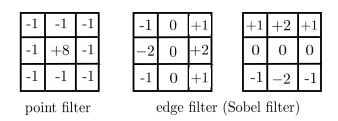
\includegraphics[width=0.4\textwidth]{./point_edge.png}
\end{figure}
In the simple case of two colors (0 and 1) this point filter would return zero for no point, 1 or -1 for a point in the outer
region and 8 or -8 if the point is in the middle. This goes analogously for the other filter.
\subsection*{d}
The first is deterministic and the second has a noise parameter and can return different states for set parameters and a given
input.


\section*{2.2}
\subsection*{a}
\begin{figure}[h]
\centering
 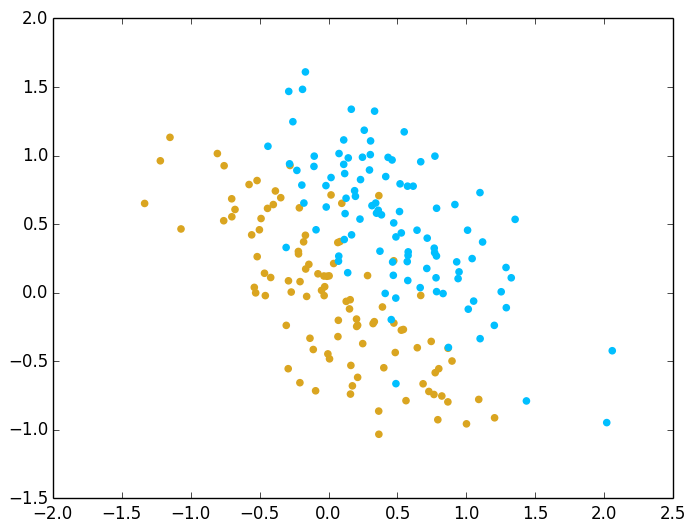
\includegraphics[width=\textwidth]{./2_2_a.png}
\caption{Plot where Y=1 (blue) and Y=0 (gold).}
\end{figure}


\subsection*{b}
\begin{figure}[h]
\centering
 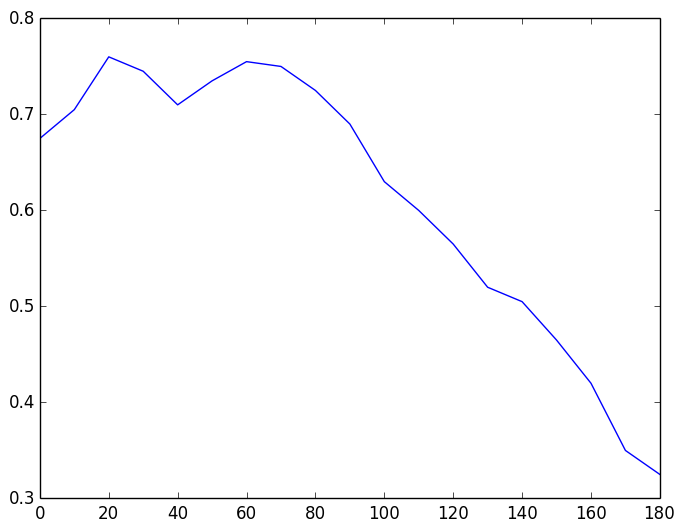
\includegraphics[width=\textwidth]{./2_2_b.png}
\caption{Classification performance for different alphas.}
\end{figure}

\subsection*{c}
Best weight vector is .

\subsection*{d}
\begin{figure}[h]
\centering
 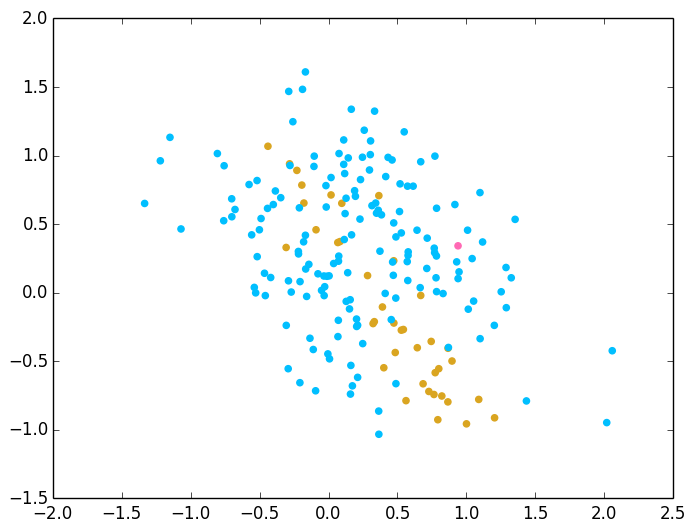
\includegraphics[width=\textwidth]{./2_2_d.png}
\caption{Classified data points. Blue = correctly classified, Gold = other data points, Pink = weight.}
\end{figure}

\subsection*{e}
\begin{figure}[h]
\centering
 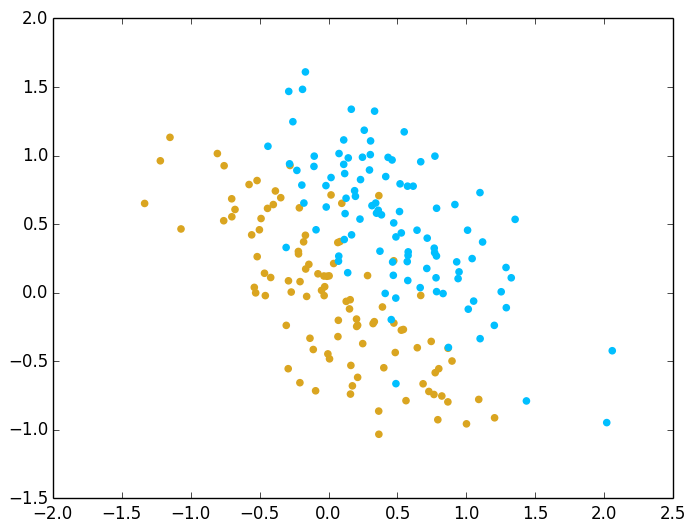
\includegraphics[width=\textwidth]{./2_2_a.png}
\caption{Plot where Y=1 (blue) and Y=0 (gold).}
\end{figure}

\section*{2.3}
\subsection*{a}
A MLP could decide between a horizontal and a vertical edge, whereas a perceptionist neuron would either be able to differ between
vertical edge or no vertical edge OR horizontal edge or no horizontal edge.
\subsection*{b}
\begin{figure}[h]
\centering
 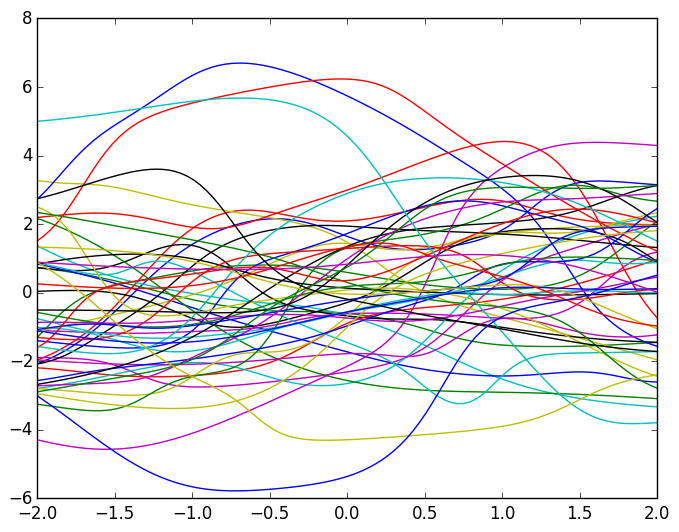
\includegraphics[width=\textwidth]{./2_3_std=2.png}
\caption{functions computed with normally distributed $a_i$ with a standard deviation of 2}
\end{figure}
\newpage
\subsection*{c + bonus}
\begin{figure}[h]
\centering
 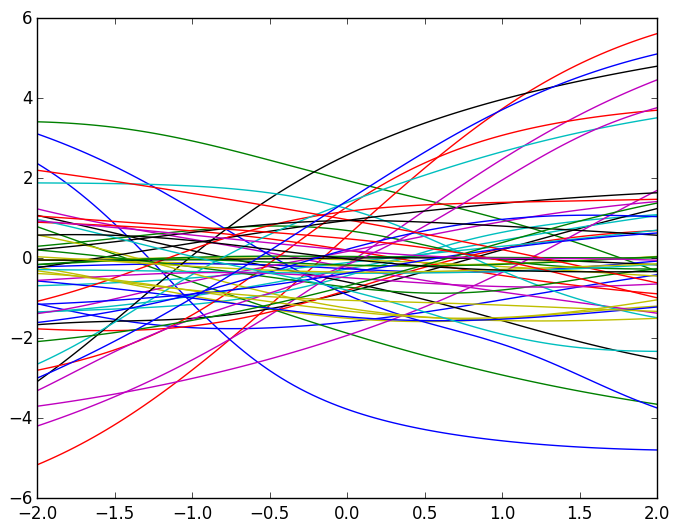
\includegraphics[width=0.75\textwidth]{./2_3_std=0_5.png}
\caption{functions computed with normally distributed $a_i$ with a standard deviation of 0.5}
\end{figure}
\begin{figure}[!h]
\centering
 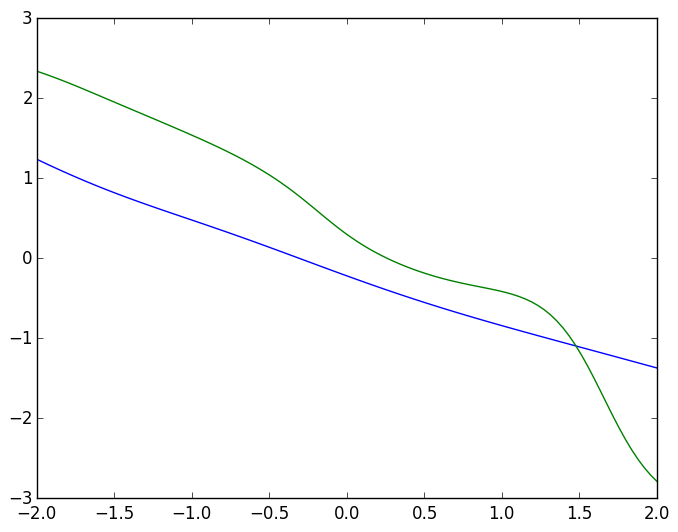
\includegraphics[width=0.75\textwidth]{./2_3_star.png}
\caption{functions with least mean square error from f(x)=-x, computed with an std of 2 (green) and 0.5 (blue)}
\end{figure}
\end{document}
